% !TEX TS-program = pdflatex
% !TEX encoding = UTF-8 Unicode

% This is a simple template for a LaTeX document using the "article" class.
% See "book", "report", "letter" for other types of document.

\documentclass[11pt]{article} % use larger type; default would be 10pt

\usepackage[utf8]{inputenc} % set input encoding (not needed with XeLaTeX)

%%% Examples of Article customizations
% These packages are optional, depending whether you want the features they provide.
% See the LaTeX Companion or other references for full information.

%%% PAGE DIMENSIONS
\usepackage{geometry} % to change the page dimensions
\geometry{a4paper} % or letterpaper (US) or a5paper or....
% \geometry{margin=2in} % for example, change the margins to 2 inches all round
% \geometry{landscape} % set up the page for landscape
%   read geometry.pdf for detailed page layout information

\usepackage{graphicx} % support the \includegraphics command and options

% \usepackage[parfill]{parskip} % Activate to begin paragraphs with an empty line rather than an indent

%%% PACKAGES
\usepackage{booktabs} % for much better looking tables
\usepackage{array} % for better arrays (eg matrices) in maths
\usepackage{paralist} % very flexible & customisable lists (eg. enumerate/itemize, etc.)
\usepackage{verbatim} % adds environment for commenting out blocks of text & for better verbatim
\usepackage{subfig} % make it possible to include more than one captioned figure/table in a single float
% These packages are all incorporated in the memoir class to one degree or another...

%%% HEADERS & FOOTERS
\usepackage{fancyhdr} % This should be set AFTER setting up the page geometry
\usepackage{cancel}
\usepackage[compat=1.0.0]{tikz-feynman} % Feynman diagram

\usepackage{amssymb} % usage of mathbb
\usepackage{amstext}
\usepackage{amsmath}

\pagestyle{fancy} % options: empty , plain , fancy
\renewcommand{\headrulewidth}{0pt} % customise the layout...
\lhead{}\chead{}\rhead{}
\lfoot{}\cfoot{\thepage}\rfoot{}

%%% SECTION TITLE APPEARANCE
\usepackage{sectsty}
\allsectionsfont{\sffamily\mdseries\upshape} % (See the fntguide.pdf for font help)
% (This matches ConTeXt defaults)

%%% ToC (table of contents) APPEARANCE
\usepackage[nottoc,notlof,notlot]{tocbibind} % Put the bibliography in the ToC
\usepackage[titles,subfigure]{tocloft} % Alter the style of the Table of Contents
\renewcommand{\cftsecfont}{\rmfamily\mdseries\upshape}
\renewcommand{\cftsecpagefont}{\rmfamily\mdseries\upshape} % No bold!

%%% END Article customizations

%%% The "real" document content comes below...

\title{CG algorithm}
\author{Jinchen}
%\date{} % Activate to display a given date or no date (if empty),
         % otherwise the current date is printed 

\begin{document}
\maketitle

\section{Motivation}

\noindent 

Conjugate gradient method is an algorithm for optimization problems. Here we just take an easy example:

\[ f(x) = \frac{1}{2}x^T Q x - x^T b, \]

in which $x$ is a vector in $\mathbb{R}^n$, $Q$ is a $n \times n$ symmetric ({\color{red}IF Q is hermitian instead of symmetric, change all T to $\dagger$}) and positive-definite matrix.

We would like to find the $x^*$ at where $f(x^*)$ has the minimum, so $f'(x^*) = Q x - b = 0$.

\begin{figure}[!th]
\begin{center}
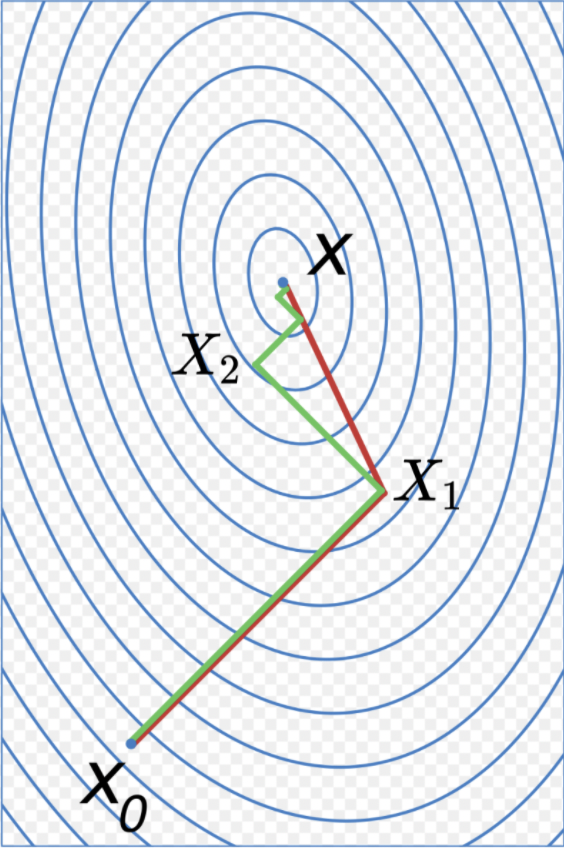
\includegraphics[width=0.4\textwidth]{fig1.png}
\caption{}
\end{center}
\end{figure}

\section{Gradient Descent}

\noindent

There is a direct way to find the minimum point of $f(x)$ which is shown by the green lines in the figure above:

\begin{itemize}
    \item Start from a random initial point $X_0$
    \item Find the negative gradient direction $d_1$
    \item Find the minimum point of $f(x)$ along that direction $d_1$ as $X_1$
    \item The next direction $d_2$ should be orthognal to the previous direction $d_1$
    \item Find the minimum point of $f(x)$ along the direction $d_2$ as $X_2$
    \item Iterate to get closer to $X^*$
\end{itemize}

There are some obvious shortages of this method: 

\begin{itemize}
    \item Zig-zag route
    \item Sepetitious steps
    \item ...
\end{itemize}

So we need another better solution\dots

\section{Conjugate Gradient Method}

\noindent

Firstly, let's give a specific definition:
\[
    \rm{d_i\ and\ d_j\ are\ Q-orthognal}: <d_i, d_j> = d_i^T Q d_j = constant \cdot \delta_ij,   
\]
then we would like to find a group of Q-orthognal basis of $\mathbb{R}^n$: $\{ d_1, d_2, \dots d_n\}$, so that we can approach $x^*$ in each direction independently.

Assume $x^* = \sum_i \alpha^*_i d_i$, then we have $b = Q x^* = \sum_i \alpha^*_i Q d_i$, multiply the equation by $d_k^T$, we select the $\alpha^*_k$ out as $\alpha^*_k = \frac{d_k^T b}{d_k^T Q d_k}$.

Now let's try to find $\{ d_1, d_2 \dots d_n \}$ and to get $x^*$.

We have an initial guess $x_1$, the negative gradient at $x_1$ is $d_1 = b - Q x_1$, calculate
\[ \alpha_1 = \frac{d_1^T d_1}{d_1^T Q d_1}, \]
then go to the next point $x_2 = x_1 + \alpha_1 d_1$.

The gradient at $x_2$ is $g_2 = Q x_2 - b$, calculate
\[ \beta_1 = \frac{g_2^T Q d_1}{d_1^T Q d_1}, \]
and the next direction is $d_2 = -g_2 + \beta_1 d_1$, which is Q-orthognal to $d_1$
\[ d_2^T Q d_1 = -g_2^T Q d_1 + \beta_1 d_1^T Q d_1 = 0, \]
so, just follow the steps above to get $d_n$,
\[\beta_k = \frac{g^T_{k+1}Qd_k}{d_k^T Q d_k}, \]
and
\[ d_{k+1} = -g_{k+1} + \beta_k d_k, \]
notice here
\[ g_k = Q x_k - b. \]

And how long should $x_k$ to go along $d_k$ to get $x_{k+1}$?

Destination:
\[ x^* = \sum_i \frac{d_i^T b}{d_i^T Q d_i} \cdot d_i = \sum_i \frac{d_i^T Q x^*}{d_i^T Q d_i} \cdot d_i \]

Where we are:
\[ x_k = \sum_i \frac{x_k^T Q d_i}{d_i^T Q d_i} \cdot d_i \]

So, 

\[ \alpha_k = \frac{d_k^T b - x_k^T Q d_k}{d_k^T Q d_k} = \frac{-g_k^T d_k}{d_k^T Q d_k} \]
and
\[ x_{k+1} = x_k + \alpha_k d_k \]

Iterate to get closer to $x^*$.

\begin{center}
    Why we need to define Q-orthognal?
\end{center}
If we choose a group of $\{d_1, d_2, \dots d_n\}$, which satisfy $d_i^T d_j = constant \cdot \delta_{ij}$, then

\[ b = \sum_i \beta_i d_i \]

\[ Qx = \sum_i \alpha_i Q d_i = \sum_i \alpha_i' d_i \]
then when we change $\alpha_i$ to move $x$ in one direction, all $\alpha_i'$ will be affected.

\section{For Lattice}

\noindent

For example, we know $S_F = Dslash^{-1}$, $Dslash$ is so big that is hard to inverse, but it is symmetric and positive-definite. Therefore, we can use CG algorithm to solve 
\[ x = S_F b, b = (Dslash) x ,\ for\ \forall b \]
just like for a random $b$, find $x^*$ s.t. $b=Q x^*$. But in order to satisfy the positive-definite condition, usually we change to solve
\[ D^{\dagger}b = (D^{\dagger}D) x \]

\begin{figure}[!th]
\begin{center}
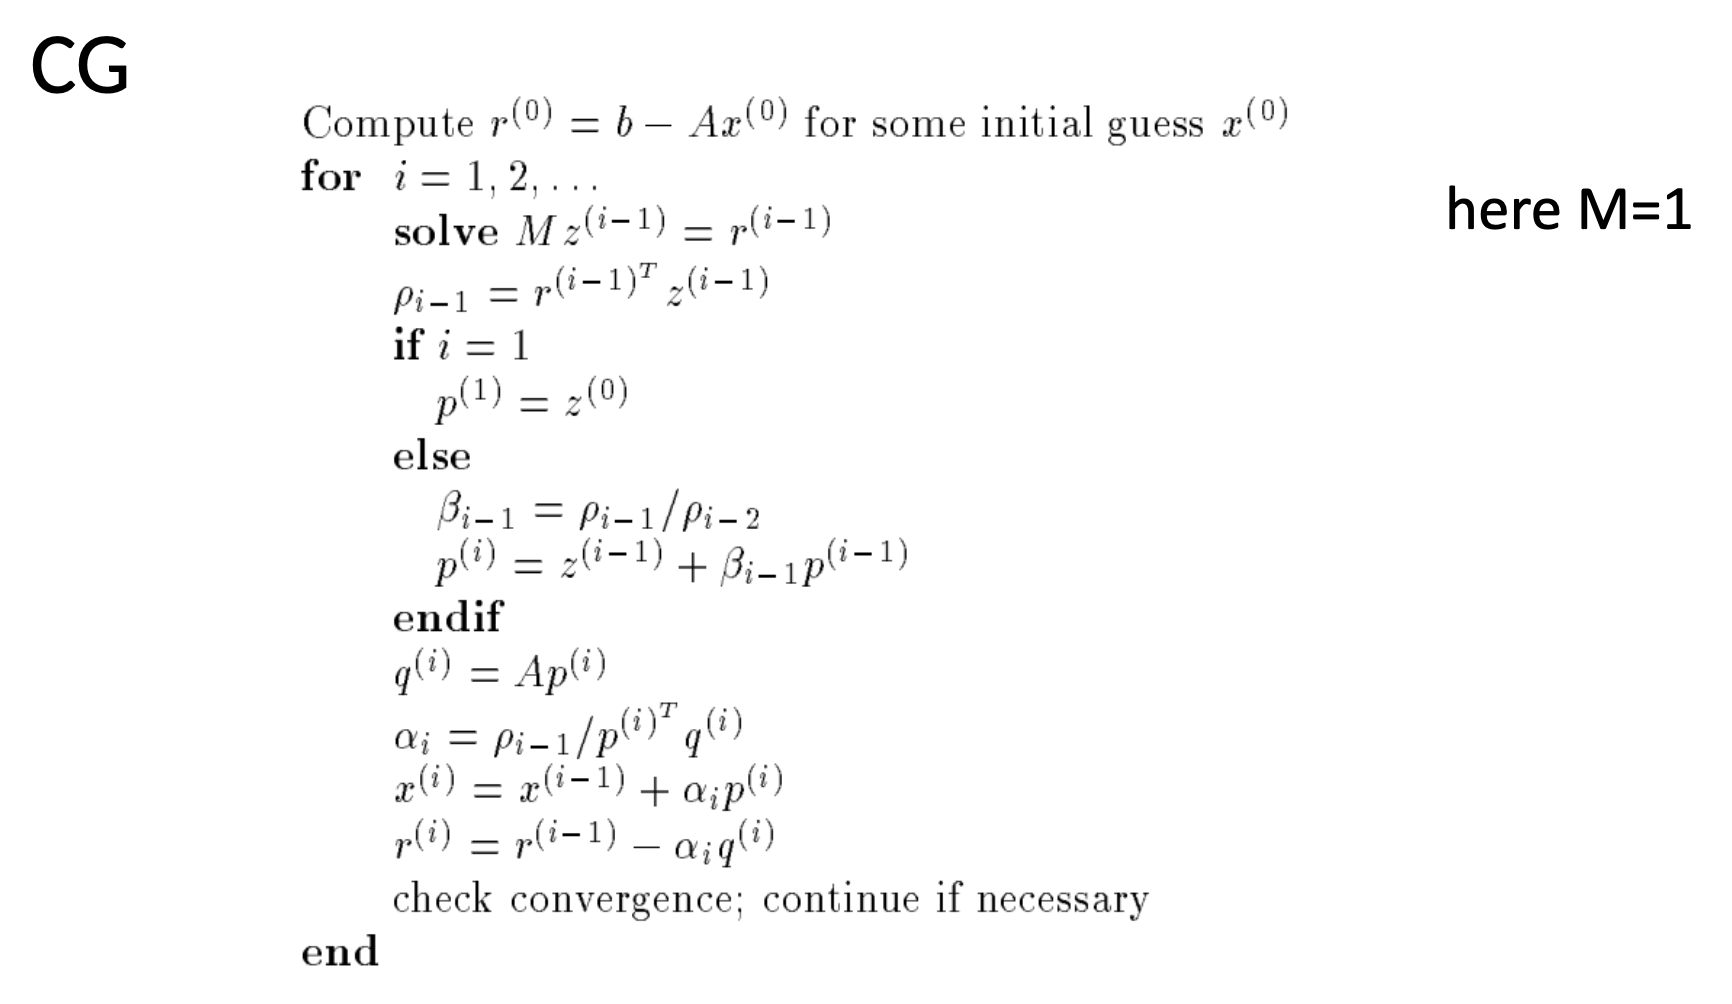
\includegraphics[width=0.9\textwidth]{fig2.png}
\caption{CG in lattice camp, from Peng Sun}
\end{center}
\end{figure}

Look at the sudo-code in the Fig.2, just adopt replacement of variables as below,

\begin{itemize}
    \item $\alpha_k \to \alpha_i$
    \item $d_k \to p^{(i)}$
    \item $-g_{k+1} \to r^{(i)}$
    \item $\beta_k \to \beta_i $
\end{itemize}

This CG algorithm has some advantages, although the length of scequences can become large, only small number of vectors need to be kept in memory. For the simple CG algorithm convergence is guaranteed for positive definite symmetric matrices, at least after N steps for matrices of dimension N, but usually significantly faster.

\section{Optimization}

\noindent

\subsection{Even-Odd Precondition}

\begin{equation}
    M=\left[\begin{array}{cc}
    M_{e e} & M_{e o} \\
    M_{o e} & M_{o o}
    \end{array}\right]
\end{equation}

\begin{equation}
    \begin{aligned}
    M &=\left[\begin{array}{cc}
    1 & 0 \\
    M_{o e} M_{e e}^{-1} & 1
    \end{array}\right] \cdot\left[\begin{array}{cc}
    M_{e e} & 0 \\
    0 & M_{o o}-M_{o e} M_{e e}^{-1} M_{e o}
    \end{array}\right] \cdot\left[\begin{array}{cc}
    1 & M_{e e}^{-1} M_{e o} \\
    0 & 1
    \end{array}\right] \\
    &=L \tilde{M} U
    \end{aligned}
\end{equation}

Therefore, $M \phi = x$ becomes $\tilde{M} \phi' = x'$, in which $\phi = U^{-1} \phi'$ and $x' = L^{-1} x$.

And we know,

\begin{equation}
    \left[\begin{array}{cc}
    1 & 0 \\
    A & 1
    \end{array}\right] \cdot\left[\begin{array}{cc}
    1 & 0 \\
    -A & 1
    \end{array}\right] = \left[\begin{array}{cc}
    1 & 0 \\
    0 & 1
    \end{array}\right]
\end{equation}

\subsection{Preconditioning methods}

\noindent

So-called preconditioning methods sometimes allow one to accelerate the convergence, depending on the Dirac operator. A preconditioner is a suitable matrix $M$ which we use to transform the system to
\[    M^{-1} A \boldsymbol{x}=M^{-1} \boldsymbol{b}. \]

Let us assume that we have a matrix $M$, which is numerically cheap to invert, i.e., to solve $M \hat{\boldsymbol{s}}=\boldsymbol{s}$ for $\hat{\boldsymbol{s}}$, and which approximates $A$ in some way. Then the spectral properties of $M^{-1} A$ may be more favorable, allowing faster convergence of the iterative solution. This may be true in particular, if the small eigenvalues of $M$ agree with those of $A$. For a more complete discussion of such methods please check:

\begin{itemize}
    \item R. Barrett et al.: Templates for the Solution of Linear Systems: Building Blocks for Iterative Methods (SIAM, Philadelphia 1994) $139,140,141$
    \item I. Montvay and G. Münster: Quantum Fields on a Lattice (Cambridge University Press, Cambridge, New York 1994) 141
\end{itemize}

\end{document}